\chapter{Modelado de un cuadricóptero}

Un cuadricóptero es un robot aéreo con 6 grados de libertad (3 rotacionales y 3 traslacionales) y 4 motores, al tener menos motores que el número de grados de libertad, se dice que es un sistema subactuado.

\begin{figure}[htb!]
	\centering
	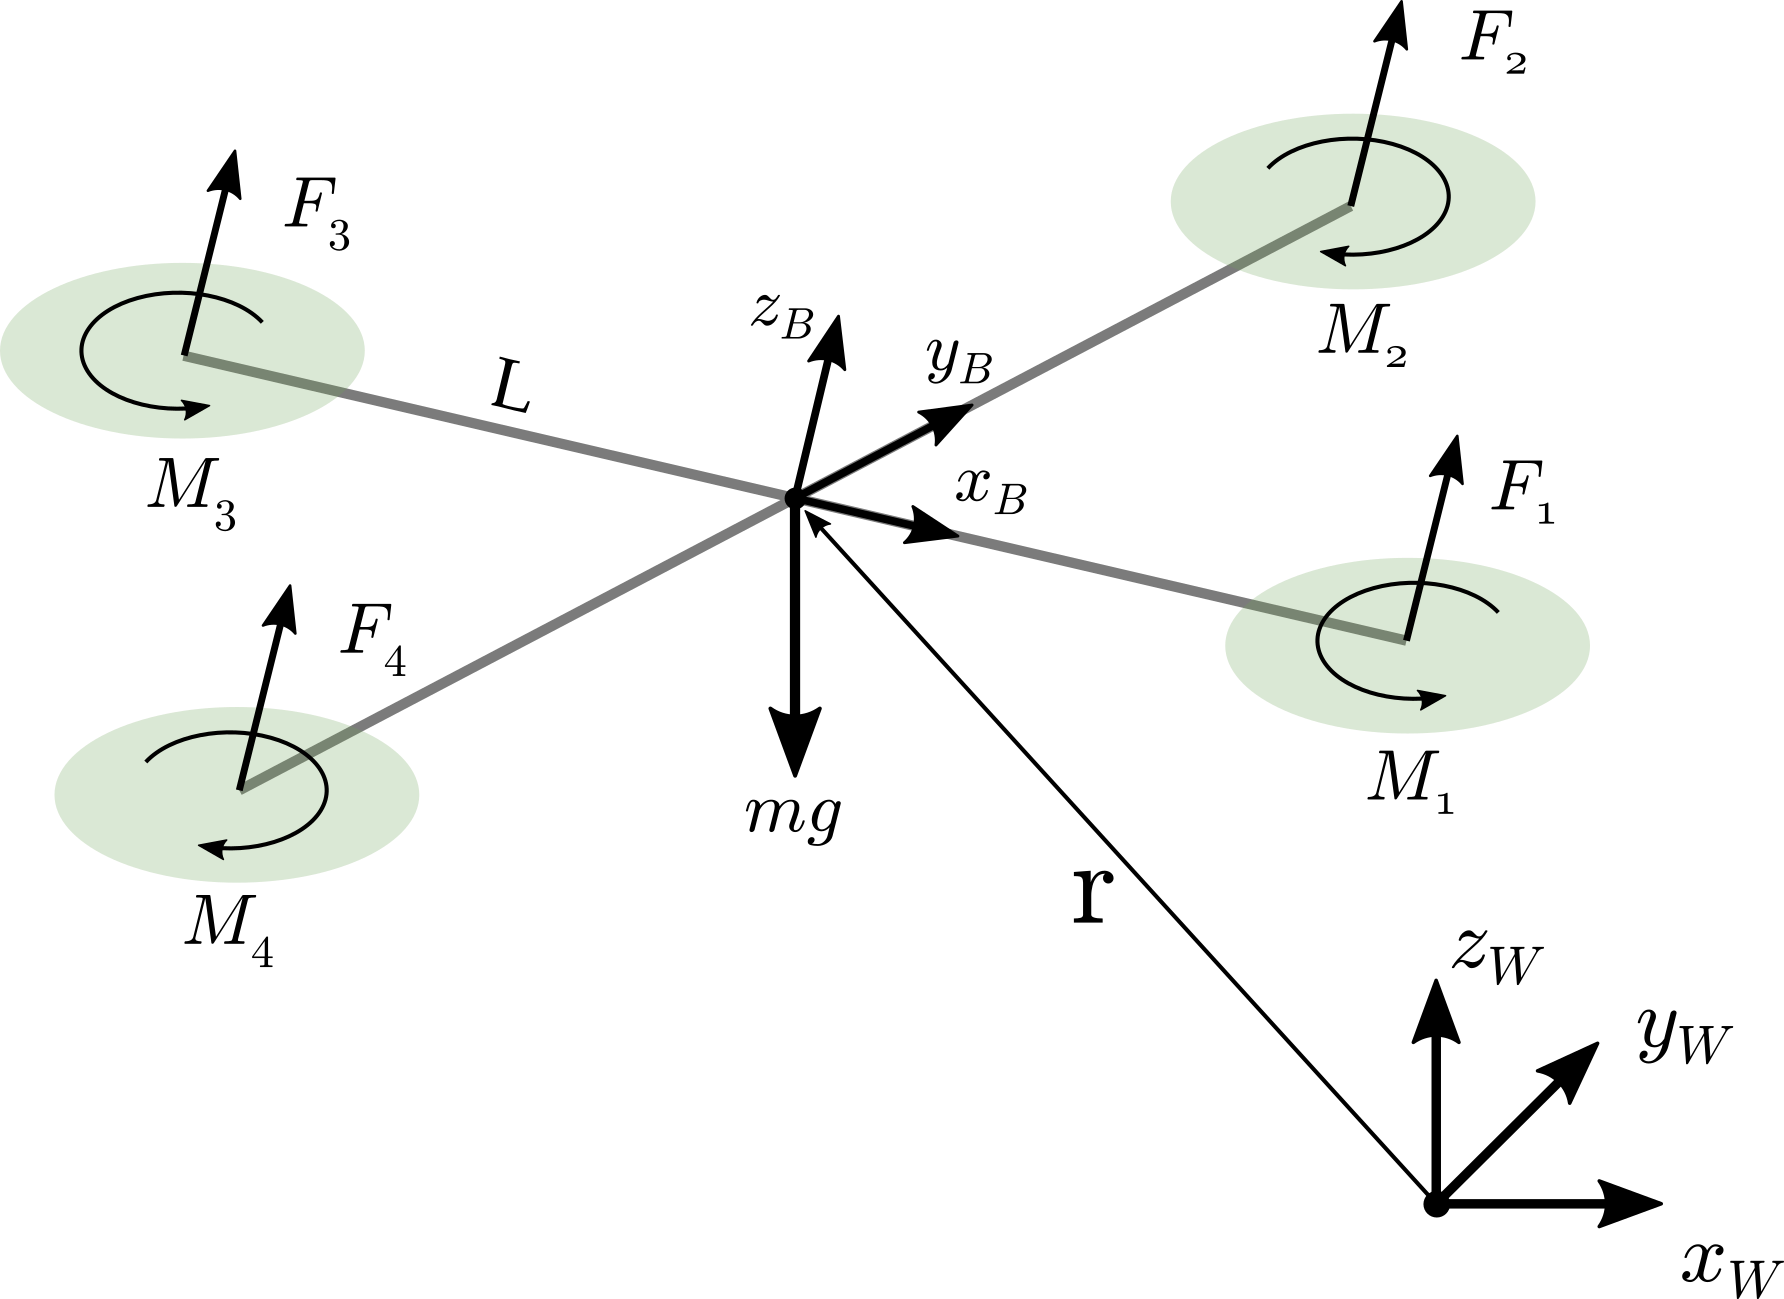
\includegraphics[width=0.65\textwidth]{imagenes/uav_coordinate_system}
	\caption{Esquema de fuerzas y momentos que actúan sobre un cuadricóptero y sus sistemas de referencia asociados. }
	\label{modelado:uav_coordinate}
\end{figure}

Como puede observar en la figura \ref{modelado:uav_coordinate}, se ha  empleado el subíndice $W$ para hacer referencia al sistema de referencia del mundo, así como el subíndice $B$ para referirse al sistema asociado al cuerpo del cuadricóptero. El \textit{frame} $B$ posee su origen $O_B$ en el centro de masas de la aeronave, con el eje $x_B$ coincidente con la dirección de avance preferente de la aeronave.

Para modelar las rotaciones del \textit{frame} $B$ con respecto a $W$ se emplearán los ángulos de Euler Z-X-Y, es decir, la matriz de rotación $R$ para transformar coordenadas desde $B$ a $W$ consiste en la composición de las siguientes rotaciones:
\begin{equation}
	R = R_{\mathbf{z},\psi}R_{\mathbf{x},\phi}R_{\mathbf{y},\theta}
	\label{modelado:euler_z_x_y}
\end{equation}
siendo $R_{\mathbf{i},\alpha}$ una rotación de un ángulo $\alpha$ respecto al eje $i$. Al desarrollar la expresión \ref{modelado:euler_z_x_y} se obtiene la matriz $R$ resultante
\begin{equation}
	\label{modelado:R}
	R = \begin{bmatrix}
		c_{\psi} c_{\theta} - s_{\phi} s_{\psi} s_{\theta} &  -c_{\phi} s_{\psi}& c_{\psi} s_{\theta} +  c_{\theta} s_{\phi} s_{\psi}\\
		c_{\theta} s_{\psi} +  c_{\psi} s_{\phi} s_{\theta} & c_{\phi} c_{\psi} & s_{\psi} s_{\theta} -  c_{\theta} s_{\phi} c_{\psi} \\
		-c_{\phi}s_{\theta}& s_{\phi} & c_{\phi}c_{\theta} 
	\end{bmatrix}
\end{equation}

donde $c_{\theta}$ y $s_{\theta}$ denotan $cos(\theta)$ y $sen(\theta)$ respectivamente.

En el sistema de referencia $B$ las componentes del vector velocidad angular $\Omega$ están definidas por $p$, $q$ y $r$ de la forma: 

\begin{equation}
	\Omega = p \mathbf{x_B} + q \mathbf{y_B} + r \mathbf{z_B}
\end{equation}

Estas componentes están relacionadas con las derivadas de los ángulos de Euler de acuerdo a

\begin{equation}
	\begin{bmatrix}
		p\\
		q\\
		r
	\end{bmatrix}  = \begin{bmatrix}
	c_{\theta}&0& -c_{\phi} s_{\theta}\\
	0 & 1 & s_{\phi}\\
	s_{\theta}&0 & c_{\phi} c_{\theta}
\end{bmatrix}\begin{bmatrix}
\dot{\phi}\\
\dot{\theta}\\
\dot{\psi}
\end{bmatrix} 
\end{equation}

\section{Análisis dinámico}
\subsection{Ecuaciones de movimiento traslacional}
Como se puede observar en la figura \ref{modelado:uav_coordinate}, las fuerzas que actúan sobre el cuadricóptero son: la gravedad, en la dirección $-\mathbf{z_W}$ y la fuerza de cada uno de los motores, en la dirección $\mathbf{z_B}$. Para hallar las ecuaciones que rigen la dinámica del centro de masas del sistema $C$ se aplican las ecuaciones de Newton sobre él. Siendo $\mathbf{r}$ el vector de posición del centro de masas $C$ con respecto al origen de $W$ obtenemos:

\begin{equation}
	\label{analisis:eq1}
	m \mathbf{\ddot{r}} = \begin{bmatrix}
		0\\
		0\\
		-mg
	\end{bmatrix} + R \begin{bmatrix}
	0\\
	0\\
	F_1+F_2 + F_3 + F_4
\end{bmatrix}
\end{equation}

Si denominamos $F  = \displaystyle\sum_{i=1}^{4}F_i$ , al expandir la ecuación anterior con la definición de $R$ en \ref{modelado:R} obtenemos las ecuaciones que describen el movimiento traslacional del centro de masas del cuadricóptero:

\begin{equation}
	\label{analisis:eq2}
	m \mathbf{\ddot{r}} = \begin{bmatrix}
		0\\
		0\\
		-mg
	\end{bmatrix} +\begin{bmatrix}
		s_{\theta}c_{\psi} + s_{\phi}c_{\theta}s_{\psi} \\
		s_{\theta}s_{\psi} - s_{\phi}c_{\theta}c_{\psi} \\
		c_{\phi}c_{\theta}
	\end{bmatrix} F
\end{equation}

\subsection{Ecuaciones de movimiento rotacional}

Como se puede observar en la expresión anterior, el movimiento del cuadricóptero depende de la rotación $R$, por lo que es necesario modelar el movimiento rotacional del mismo. Se define el momento angular $H$ como:
\begin{equation}
	H = \mathbf{I}\Omega
\end{equation}
donde $\mathbf{I} \in \mathbb{R}^{3\times 3}$ representa el tensor de inercia del cuadricóptero en el sistema $B$, y $\Omega  = [p, q, r]$ representa el vector de velocidad angular de $B$ respecto $W$. 

Si denotamos $M_c = [\tau_x, \tau_y, \tau_z]^t$ como el momento total del cuadricóptero en el sistema $B$

\begin{align}
	M_c &= \frac{d}{dt}H\nonumber\\
		&= \mathbf{I}\dot{\Omega}+\Omega\times\mathbf{I}\Omega
	\label{model:rot1}
\end{align}

Se considera que el cuadricóptero presenta una distribución de masa simétrica, por lo que el tensor de inercia $\mathbf{I}$ es un tensor diagonal de la forma:

\begin{equation}
	\mathbf{I} = \begin{bmatrix}
		I_{xx}&0&0\\
		0&I_{yy}&0\\
		0&0&I_{zz}\\
	\end{bmatrix}
\end{equation}
siendo $I_{xx}$, $I_{yy}$, $I_{zz}$ los momentos principales del cuadrícoptero con respecto a los ejes $x_B$, $y_B$, $z_B$ respectivamente.

Desarrollando la expresión \ref{model:rot1} y reorganizando sus términos:
\begin{align}
\mathbf{I}\begin{bmatrix}
	\dot{p}\\
	\dot{q}\\
	\dot{r}
\end{bmatrix}=
\begin{bmatrix}
	\tau_x\\
	\tau_y\\
	\tau_z
\end{bmatrix} -\begin{bmatrix}
	p\\
	q\\
	r
\end{bmatrix} \times\mathbf{I}\begin{bmatrix}
	p\\
	q\\
	r
\end{bmatrix}\label{model:rot2}
\end{align}

A partir del diagrama de la figura \ref{modelado:uav_coordinate} se puede calcular los valores de $\tau_x$, $\tau_y$ y $\tau_z$ a partir de las fuerzas y momentos ejercidos por los motores.

\begin{align}
	\tau_x &=  L (F_2-F_4)\nonumber\\
	\tau_y &=  L (F_3-F_1)\nonumber\\
	\tau_z &=  M_1 - M_2 + M_3 - M_4\label{model:rot3}
\end{align}

Finalmente se unen las expresiones \ref{model:rot2} y \ref{model:rot3} para obtener la ecuación de movimiento rotacional del cuadricóptero.
\begin{align}
	\label{model:rot_eq}
	\mathbf{I}\begin{bmatrix}
		\dot{p}\\
		\dot{q}\\
		\dot{r}
	\end{bmatrix}=\left[
	\begin{array}{c}
		L (F_2-F_4)\\
		L (F_3-F_1)\\
		M_1 - M_2 + M_3 - M_4
	\end{array}\right] -\begin{bmatrix}
		p\\
		q\\
		r
	\end{bmatrix} \times\mathbf{I}\begin{bmatrix}
		p\\
		q\\
		r
	\end{bmatrix}
\end{align}


\section{\tb{Differential flatness}}


\chapter{Control}
En este capítulo se desarrollará la teoría general para el control de un cuadricóptero \tb{Citar artículos a cholón}, la cual se adaptará posteriormente al caso particular de la arquitectura empleada.\\

El problema del control se puede expresar formalmente: 
Dado el estado del sistema $x(t)$ \tb{continuar . ... }
como encontrar la función $u(t)$ tal que, el estado $x(t)$ sigue la trayectoria desesada $x^{des}(t)$ a lo largo del tiempo.\\
Si se define el error $e(t)$ del control como:
\begin{equation}
	e(t) = x^{des}(t) - x(t)
\end{equation}
el objetivo del controlador sería conseguir que el error $e(t)$ converja de forma exponencial a 0.


El estado $x(t)$ de un cuadricóptero consta de 12 variables, las 6 correspondientes a su pose y sus derivadas correspondientes.
\begin{equation}
	x(t) = \left[
	x  \;\;
	y  \;\;
	z  \;\;
	\phi  \;\;
	\theta  \;\;
	\psi  \;\;
	\dot{x}  \;\;
	\dot{y}  \;\;
	\dot{z}  \;\;
	\dot{\phi}  \;\;
	\dot{\theta}  \;\;
	\dot{\psi}\;\right]^t
\end{equation}
Si llamamos $q$ al vector de configuración formado por las 6 primeras variables:
\begin{align}
	q(t) &= \left[
	x  \;\;
	y  \;\;
	z  \;\;
	\phi  \;\;
	\theta  \;\;
	\psi  \;\right]^t\\
	x(t) &= \left[q \;\; \dot{q}\right]^t
\end{align}

Para el control de la aeronave se han definido dos señales de entrada $\mathbf{u_1}$ y $\mathbf{u_2}$ siendo 
\begin{align}
	\mathbf{u_1}  &= F =  F_1 +F_2 +F_3 +F_4  \label{eq:u1}\\
	\mathbf{u_2}  &= \begin{bmatrix} \tau_x\\ 
		\tau_y\\
		\tau_z
	\end{bmatrix} =\begin{bmatrix}
	L (F_2-F_4)\\
	L (F_3-F_1)\\
	M_1 - M_2 + M_3 - M_4
\end{bmatrix}
\end{align} 
como se puede observar la señal de control $u_1$ actúa sobre el empuje total de la aeronave en el eje $z_B$ mientras la señal $u_2$ controla los momentos totales aplicados sobre el cuadricóptero. Los pares $M_i$ que ejerce cada motor se relacionan con $F_i$ de la forma $M_i = \gamma F_i$, siendo $\gamma$ una constante aerodinámica dependiente de las hélices empleadas. De esta forma se puede expresar $u_2$ de la siguiente forma:

\begin{align}
	\mathbf{u_2}  &= \begin{bmatrix}
		0&L&0&-L\\
		-L&0&L&0\\
		\gamma&-\gamma&\gamma&-\gamma\\
	\end{bmatrix}\begin{bmatrix} F_1\\ 
	F_2\\ 
	F_3\\ 
	F_4\\ 
\end{bmatrix}\label{eq:u2}
\end{align} 

La arquitectura de control general consiste en dos controladores anidados: un controlador de posición y un controlador de orientación, como se puede observar en la figura .\tb{incluir diagrama}




\section{Controlador para ángulos pequeños}
Cuando las trayectorias que el cuadricóptero son poco agresivas se puede linealizar el modelo del cuadricóptero entorno a su punto de equilibrio. En la situación de equilibrio el cuadricóptero se encuentra en \textit{hover}, es decir manteniendo la posición en el aire . En \textit{hover} el estado $x_0$ de la aeronave es de la forma 
\begin{align}
	x_0 &= [q_0 \;\; 0]^t\nonumber\\
	q_0 &= [x_0  \;\;y_0  \;\;z_0  \;\;0  \;\;0  \;\;\psi_0  \;]^t
\end{align}
Como los ángulos $\phi$ y $\theta$ son pequeños se puede aproximar $cos(\phi) \approx 1 , cos(\theta) \approx 1$ y $sen(\phi) \approx \phi , sen(\theta) \approx \theta$. En este estado de equilibrio la fuerza total que ejercen los motores debe ser igual al peso del cuadricóptero por lo que:
\begin{equation}
	F_{i,0}  = \frac{mg}{4}\quad,\quad \mathbf{u_{1,0}} = mg
\end{equation}

Al desglosar y linealizar las ecuaciones \ref{analisis:eq2} entorno a este estado obtenemos las ecuaciones linealizadas del movimiento traslacional:
\begin{align}
	\ddot{x} &= g (\Delta\theta\, cos \psi_0 + \Delta\phi\,sen\psi_0)\nonumber \\
	\ddot{y} &= g(\Delta\theta\, sen \psi_0  - \Delta\phi\,cos\psi_0) \label{eq:control1}\\
	\ddot{z} &= \frac{1}{m}\mathbf{u_1}-g\nonumber
\end{align}

Por otro lado, para obtener las ecuaciones que permiten controlar la rotación del cuadricóptero debemos desarrollar las ecuaciones \ref{model:rot_eq}. Debido a la simetría del cuadricóptero se considera que $I_{xx} \approx I_{yy}$, con lo que se obtienen las ecuaciones del movimiento rotacional:
\begin{align}
	I_ {xx} \dot p &= u_2 - qr(I_{zz}-I_{yy})\nonumber\\
	I_ {yy} \dot q &= u_3 - pr(I_{xx}-I_{zz})\label{eq:control2}\\
	I_ {zz} \dot r &= u_4\nonumber
\end{align}
Se puede asumir que la componente r es pequeña por lo que los productos de esta con otros términos, también son pequeños en comparación con el resto de términos. Además, en el estado de \textit{hover} $\dot{\phi}\approx p$, $\dot{\theta}\approx q$ y $\dot{\psi}\approx r$. Es por esto que la expresión anterior se puede simplificar por:
\begin{align}
	\dot p &= \frac{u_2}{I_ {xx}} \nonumber\\
	\dot q &= \frac{u_3}{I_ {yy}}\label{eq:control3}\\
	\dot r &= \frac{u_4}{I_ {zz}}\nonumber
\end{align}
Gracias a esto es posible expresar el valor de las acciones de control $\mathbf{u_2}$ como:
\begin{align}
	\label{eq:u2_linearized}
	u_{2,des} &= k_{p,\phi}(\phi^{des}-\phi) + k_{d,\phi}(p^{des}-p)\\
	u_{3,des} &= k_{p,\theta}(\theta^{des}-\theta) + k_{d,\theta}(q^{des}-q)\\
	u_{4,des} &= k_{p,\psi}(\psi^{des}-\psi) + k_{d,\psi}(r^{des}-r)
\end{align}

En el estado de hover,las velocidades de roll y pitch son cero por lo que $p_{des} = 0\;, q_{des} = 0$.

\subsection{Controlador de posición}


En cuanto al tipo de controlador se ha decidido emplear un controlador PD. En un controlador PD el objetivo de seguir la trayectoria $r_T$ deseada es conseguir que la expresión \ref{pd:1} tienda a 0 en un tiempo exponencial:
\begin{equation}
	\label{pd:1}
	\left(\ddot{r_T} - \ddot{r_c}\right) + K_d e_v + K_p e_p = 0
\end{equation}
siendo $e_v = (\dot r_T - \dot r_c )$ y $e_p = (r_T - r_c )$. Las constantes $K_d,K_p \in \mathbb{R^+}$ del controlador definen la dinámica y la estabilidad del sistema.

Desarrollando \ref{pd:1}:
\begin{align}
	\label{pd:2}
	\ddot{r_c} = \ddot{r_T} + K_d e_v + K_p e_p
\end{align}

Al combinar \ref{eq:control1} con \ref{pd:2}:
\begin{align}\begin{bmatrix}
		g (\Delta\theta\, cos \psi_0 + \Delta\phi\,sen\psi_0)\\
		g(\Delta\theta\, sen \psi_0  - \Delta\phi\,cos\psi_0) \\
		\frac{1}{m}\mathbf{u_1}-g
	\end{bmatrix} 	= \ddot{r_T} + K_d e_v + K_p e_p
\end{align}

por lo que :
\begin{align}
	\mathbf{u_1} &=m\left(g + \ddot{z_{des}}+ K_{d,z}(\dot{z_{des}}-\dot{z}) + K_{p,z}(z_{des}-z)\right)\\
	\phi^{des} &= \frac{1}{g}\left(\ddot{x}_{des} sin\,\psi_T -\ddot{y}_{des} cos\,\psi_T \right)\\
	\theta^{des} &= \frac{1}{g}\left(\ddot{x}_{des} cos\,\psi_T +\ddot{y}_{des} sin\,\psi_T \right)
\end{align}

Como el angulo de \textit{yaw} $\psi_T(t)$ se incluye en la trayectoria definida, entonces:
\begin{align}
	\psi_{des} &= \psi_T(t)\\
	r_{des} &= \dot\psi_T(t)
\end{align} 

\tb{ completar un poco más }

\section{Controlador para ángulos grandes}
A continuación se presenta un controlador que no parte de la premisa de que el estado de la aeronave es cercano al de equilibrio y que permite seguir trayectorias $\sigma_T = [\mathbf{r}_T(t)^t, \psi_T(t)]^t$.

El objetivo de este controlador es orientar el vector $z_B$ de la aeronave con la dirección de la fuerza necesaria $\mathbf{F}_{des}$ para poder seguir la trayectoria.
\tb{imagen}

Para ello primero definiremos los errores en posición y velocidad:
\begin{align}
	\mathbf{e}_p &= \mathbf{r} -\mathbf{r}_T\\
	\mathbf{e}_v &= \mathbf{\dot r} -\mathbf{\dot r}_T
\end{align} 

La fuerza deseada $\mathbf{F}_{des}$ en cada instante de tiempo viene dada por la expresión
\begin{equation}
	\mathbf{F}_{des} = -K_p	\mathbf{e}_p - K_v	\mathbf{e}_v - mg	\mathbf{z}_W + m	\mathbf{\ddot r}_T
\end{equation}
donde $K_p$ y $K_v$ son matrices definidas positivas.
Como se puede observar, la fuerza debe tener en cuenta el peso de la aeronave, la aceleración impuesta por la trayectoria en ese instante y el error de seguimiento de la trayectoria en ese instante para poder corregirlo.

Al proyectar $\mathbf{F}_{des}$ sobre el eje $x_B$ del cuadricóptero se puede obtener $u_1$, por lo que:
\begin{equation}
	u_1,des = \mathbf{F}_{des}\cdot \mathbf{z}_B
\end{equation}

Las otras tres señales de control del sistema dependen de la orientación de la aeronave. El objetivo es alinear el eje $\mathbf{z}_B$ de la aeronave con la dirección de la fuerza deseada $\mathbf{z}_{B,des}$, es decir, que la matriz de rotacion $R_{des}$ viene dada por:
\begin{align}	
	R_{des}\mathbf{e_3} = \mathbf{z}_{B,des}\;,\quad 
\mathbf{z}_{B,des} = \frac{\mathbf{F}_{des}}{||\mathbf{F}_{des}||}
\end{align}
siendo $\mathbf{e_3}$ el vector director del eje $z_B$ de la aeronave respecto al sistema $B$, es decir, $\mathbf{e_3} = [0, 0, 1]^t$.
Debido a que el ángulo de yaw $\psi_T$ viene dado por la trayectoria se pueden calcular los vectores de rotación deseados de la forma:
\begin{gather}
	\mathbf{x}_{C,des} = [cos\, \psi_T , sin \psi_T, 0]^t\\
	\mathbf{y}_{B,des} = \frac{\mathbf{z}_{B,des}\times\mathbf{x}_{C,des}}{||\mathbf{z}_{B,des}\times\mathbf{x}_{C,des}||}\;,\; \mathbf{x}_{B,des} = \mathbf{y}_{B,des} \times\mathbf{z}_{B,des}
\end{gather}
por lo que la matriz $R_{des} \in SO(3)$ se expresa como:
\begin{equation}
	R_{des}=
	\begin{bmatrix}
		\vrule&\vrule&\vrule\\
		\mathbf{x}_{B,des}&\mathbf{y}_{B,des}&\mathbf{z}_{B,des}\\
		\vrule&\vrule&\vrule
	\end{bmatrix}
\end{equation}

A continuación definiremos el error en orientación como:
\begin{equation}
	\mathbf{e}_R = \frac{1}{2}\left(R_{des}^t R - R^t R_{des} \right)^\vee
\end{equation}
donde $\vee$ denota el \tb{vee map} que transforma elementos de $SO(3)$ a $\mathbb{R}$. El error de velocidad angular es simplemente la diferencia entre la velocidad angular de la aeronave y la velocidad angular deseada, ambas medidas con respecto las coordenadas del sistema de coordenadas del cuadricóptero $B$.
\begin{equation}
	\mathbf{e}_\omega = \null^B[\omega]-\null^B[\omega_T] 
\end{equation}
Finalmente, las tres señales de salida restantes, correspondientes con los pares ejercidos sobre la aeronave, se calculan como:

\begin{equation}
	\label{eq:u2_non_linearized}
\begin{bmatrix}
	u_{2,des}\\u_{3,des}\\u_{4,des} 
\end{bmatrix}= -K_R	\mathbf{e}_R - K_\omega	\mathbf{e}_\omega
\end{equation}

Este controlador presenta dos ventajas considerables con respecto al controlador anterior:
\begin{enumerate}
	\item El error en orientación está expresado mediante matrices de rotación y no mediante ángulos de Euler, los cuales presentan una singularidad en torno a $\theta = 90º$ conocida como \textit{gimbal lock}.
	\item La fuerza deseada se proyecta sobre el vector $z_B$ de la aeronave en el instante actual, en lugar de considerar que éste siempre apunta verticalmente, por lo que mejora notablemente el control en trajectorias agresivas, donde la aeronave presenta una gran inclinación.
\end{enumerate}

\tb{hablar de la estabilidad y robustez del sistema}

\section{Adaptación del controlador al entorno simulado.}

En los controladores anteriores las señales de salida están directamente relacionadas con la velocidad de giro de cada motor y de la fuerza de empuje que genera cada uno, como se puede observar en las expresiones \ref{eq:u1} y \ref{eq:u2}. Sin embargo, en la competición, no se tiene el control de cada motor de forma independientemente, si no que hay un controlador interno que controla los motores. Es por esto que, es necesario adaptar los controladores del estado del arte mostrados anteriormente al nuevo conjunto de señales de entrada disponibles.

\tb{diagrama nuevo}

El controlador interno del cuadricóptero tiene como consignas a seguir las velocidades angulares del cuadrícoptero deseadas, así como el empuje total que deben proporcionar los motores. Estas son las señales que envían los pilotos de carreras de drones profesionales a través de sus mandos, debido al gran control que tienen de la aeronave. Al poder controlar el empuje total de la aeronave, la señal $u_1$ se mantiene igual que en los controladores anteriores, sin embargo es necesario realizar algunas pequeñas modificaciones en los controladores angulares. Las otras 3 señales de control que se van a emplear son las referencias del controlador interno $p_{ref}$,$q_{ref}$ y $r_{ref}$.

\subsubsection{Modificaciones para ángulos pequeños}
Como se puede observar en la expresión \ref{eq:u2_linearized},  el controlador angular es un control PD que depende de la orientación actual de la aeronave y de la orientación deseada. Dado que el objetivo es minimizar ese error de orientación, podemos expresar el controlador angular como:
\begin{align}
	u_2 = p_{ref} &=  p_{des} + k_{p,\phi}(\phi^{des}-\phi)\\
	u_3 = q_{ref} &=  q_{des} + k_{p,\theta}(\theta^{des}-\theta)\\
	u_4 = r_{ref} &=  r_{des} + k_{p,\psi}(\psi^{des}-\psi)
\end{align}


\subsubsection{Modificaciones para ángulos grandes}
Para el controlador para grandes ángulos se ha aplicado una estrategia similiar a la anterior. La expresión \ref{eq:u2_non_linearized} se ha modificado para que sea de la forma:
\begin{equation}
	\begin{bmatrix}
		u_{2}\\u_{3}\\u_{4} 
	\end{bmatrix}=\null^B[\omega] =  \null^B[\omega_T]    -K_R	\mathbf{e}_R  
\end{equation}
\\

Con estas pequeñas modificaciones se ha conseguido adaptar los controladores del estado del arte al interfaz provisto por el entorno de simulación que se empleará posteriormente en los experimentos.


